\documentclass{beamer}

\usepackage{beamerthemeSingapore}
\usepackage{graphicx}
%\usepackage{here}
\usepackage{url}
\usepackage[brazil]{babel}
\usepackage[utf8]{inputenc}
\usepackage[tight,raggedright]{subfigure}
%usepackage[alf]{abntex2cite}
\usepackage{listings}
\usepackage{minted}
\usepackage{amsmath}
\usepackage{pdfpages}
% Please add the following required packages to your document preamble:
\usepackage{booktabs}

% TODO TODO TODO TODO TODO TODO TODO
\title{02 - Análise de Algoritmos}
\author{Prof. Alex Kutzke}
\date{Maio de 2021}

\begin{document}

	% ==========================================
	\begin{frame}
		\begin{center}
			% TODO TODO TODO TODO TODO TODO
			\large{Setor de Educação Profissional e Tecnológica}\\
			Tecnologia em Análise e Desenvolvimento de Sistemas\\
			\vspace{1cm}			
			\small{DS143 - Estruturas de Dados II}
		\end{center}
		\titlepage
	\end{frame}
	% ==========================================

	% ==========================================
	\begin{frame}[c]{Roteiro}
		\tableofcontents
	\end{frame}
	% ==========================================

	\section{Caixeiro Viajante}
	
	% ==========================================
	\begin{frame}
		\frametitle{Problema do Caixeiro Viajante}
	
	  \begin{block}{Definição}
		Suponha que um caixeiro viajante tenha de visitar n cidades diferentes, iniciando e encerrando sua viagem na primeira cidade. Suponha, também, que não importa a ordem com que as cidades são visitadas e que de cada uma delas pode-se ir diretamente a qualquer outra. O problema do caixeiro viajante consiste em descobrir a rota que torna mínima a viagem total. 
	  \end{block}
	\end{frame}
	% ==========================================

	% ==========================================
	% Exemplo de frame com figura
	\begin{frame}
		\frametitle{Problema do Caixeiro Viajante}
	  \begin{figure}[h]
	  	\centering
	  	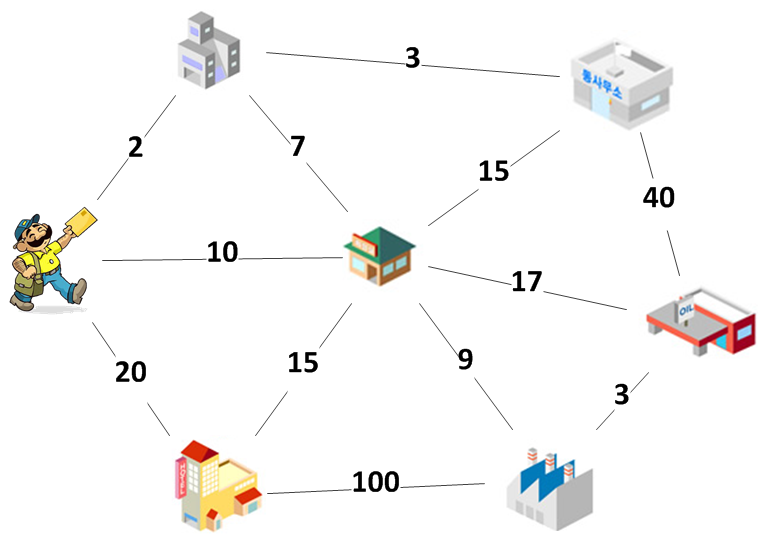
\includegraphics[width=8cm]{fig/mapa.png}
			\caption{Problema do Caixeiro Viajante.}
	  	\label{label}
	  \end{figure}
	\end{frame}
	% ==========================================

	% ==========================================
	\begin{frame}
		\frametitle{Problema do Caixeiro Viajante}
	
	  \begin{center}
			Qual a solução mais \underline{simples} para esse problema??\\
		  \pause
	  	Verificar \textbf{todas as possibilidades}.
 	  \end{center}
	\end{frame}
	% ==========================================

	% ==========================================
	\begin{frame}[t]
		\frametitle{Problema do Caixeiro Viajante}
	
	  \begin{center}
			Considere o problema com 4 cidades ($n=4$):
			$A$, $B$, $C$ ,$D$.\\ Quais são as possibilidades?
		  \pause
 	  \end{center}
 	  \begin{enumerate}
			\item ABCDA
			\item ABDCA
			\item ACBDA
			\item ACDBA
			\item ADBCA
			\item ADCBA
 	  \end{enumerate}
 	  \pause
 	  E para 5 cidades, quantas rotas são possíveis? E para 6 cidades?
 	  \pause
 	  \center{\textbf{$R(n) = (n-1)!$}}

	\end{frame}
	% ==========================================

	% ==========================================
	\begin{frame}[t]
		\frametitle{Análise do Problema}
		\begin{itemize}
			\item Clássico problema de \textbf{otimização combinatória};
			\item Solução anterior, reduz para um \textbf{problema de enumeração} e consegue encontrar a solução ótima;
		\end{itemize}
		
		Legal! Encontramos a solução. Então por que estamos falando desse problema?\\
		\pause
		Qual o problema dessa solução? \pause 

		\vspace{2cm}

		\begin{center}		
			O esforço cresce em uma taxa \textbf{fatorial}!
		\end{center}
	\end{frame}
	% ==========================================
	
	% ==========================================
	\begin{frame}[t]
		\frametitle{Análise do Problema}
		Suponha:
		\begin{itemize}
			\item Um computador muito veloz capaz de fazer 1 bilhão de adições por segundo;
			\item Um problema com 20 cidades.
		\end{itemize}
		
		O computador precisa de apenas 19 adições para dizer qual o comprimento de uma rota. Portanto:
		\begin{itemize}
			\item É capaz de calcular $10^9 / 19 = $\textbf{53 milhões de rotas por segundo};
			\item Ótimo, não?
		\end{itemize}		 
		
		Sabemos que o computador precisará calcular $19!$ rotas. Quanto é $19!$?
		\pause
		\begin{center}
		$121645100408832000$
		\end{center}
		\pause
		Assim, o computador precisará de 

		\begin{center}
		
		$1.2 \times 10^{17} / ( 53 $milhões$ ) = 2.3 x 10^9$ segundos
		\end{center}

	\end{frame}
	% ==========================================	
	
	
	% ==========================================
	\begin{frame}[t]
		\frametitle{Análise do Problema}
		\begin{center}
		
		$2.3 x 10^9$ segundos\\ 
		$ = 2300000000$ segundos\\
		\pause
		$ = 38333333$ minutos\\
		\pause
		$ = 638888$ horas\\
		\pause		 
		$ = 26620$ dias\\
		\pause
		$ = 73$ \textbf{anos}!\\
		\pause
		\end{center}
		
		``Ah, mas tudo bem! É só alocar mais processamento. Se tivermos um computador 1000 vezes mais rápido,
		quanto tempo leva?''

		\pause
		
		\begin{center}
		$73$ anos $ / 1000 = 0,073$ anos $ = 26$ dias\\		
		\end{center}

		\pause
		
		Com esse novo computador e uma única cidade a mais, já levaríamos mais de um ano para calcular a melhor rota.

	\end{frame}
	% ==========================================	


	% ==========================================
	\begin{frame}[t]
		\frametitle{Análise do Problema}
\begin{table}[]
\centering
\caption{Crescimento Fatorial.}
\label{my-label}
\begin{tabular}{@{}llll@{}}
\toprule
\multicolumn{1}{c}{\textbf{n}} & \multicolumn{1}{c}{\textbf{rotas por segundo}} & \multicolumn{1}{c}{\textbf{( n - 1 )!}} & \multicolumn{1}{c}{\textbf{cálculo total}} \\ \midrule
5                              & 250 milhoes                                    & 24                                      & insignific                                 \\
10                             & 110 milhoes                                    & 362 880                                 & 0.003 seg                                  \\
15                             & 71 milhoes                                     & 87 bilhoes                              & 20 min                                     \\
20                             & 53 milhoes                                     & 1.2 x $10^{17}$                              & 73 anos                                    \\
25                             & 42 milhoes                                     & 6.2 x $10^{23}$                              & 470 milhoes de anos                        \\ \bottomrule
\end{tabular}
\end{table}	
	\end{frame}
	% ==========================================		
	
	

	% ==========================================
	\begin{frame}[t]
		\frametitle{Análise do Problema}

\begin{table}[]
\centering
\caption{Crescimento Polinomial}
\label{my-label}
\begin{tabular}{@{}llll@{}}
\toprule
\textbf{n} & \textbf{rotas por segundo} & \textbf{$n^5$} & \textbf{cálculo total} \\ \midrule
5          & 250 milhoes                & 3 125        & insignific             \\
10         & 110 milhoes                & 100 000      & insignific             \\
15         & 71 milhoes                 & 759 375      & 0.01 seg               \\
20         & 53 milhoes                 & 3 200 000    & 0.06 seg               \\
25         & 42 milhoes                 & 9 765 625    & 0.23 seg               \\ \bottomrule
\end{tabular}
\end{table}
	\end{frame}
	% ==========================================		
	
	\section{Problemas Complexos}
	
	% ==========================================
	\begin{frame}[t]
		\frametitle{Problemas Complexos}
		
		E o que tudo isso quer dizer??
		\pause
		
		\begin{center}
			Que nem todos os problemas são facilmente resolvidos de maneira satisfatória por um computador.
		\end{center}
		
		\pause
		Mas não existe um algoritmo melhor?
		\pause
		
		
		\begin{center}
			Algoritmo ótimo? A princípio não. Se você descobrir, pode se considerar um milionário. :)
		\end{center}
		

	\end{frame}
	% ==========================================		

	% ==========================================
	\begin{frame}[t]
		\frametitle{Classes de problemas}
			
		De uma maneira \textbf{\textit{muito simplificada}}, podemos dividir problemas em 2 grupos:			
			
		\begin{block}{Problemas \textbf{P}}
		Problemas resolvíveis em tempo polinomial (de acordo com o tamanho da entrada).
		\end{block}
		
		
		\begin{block}{Problemas \textbf{NP}}
		Problemas \textbf{não} resolvíveis em tempo polinomial (de acordo com o tamanho da entrada).
		\begin{itemize}
			\item \textit{``Non-deterministic polynomial time''};
			\item Mas verificáveis em tempo polinomial;
			\item Redução de problemas;
		\end{itemize}
		\end{block}
				
		\begin{center}
			\textbf{P = NP ??}
		\end{center}
	\end{frame}
	% ==========================================			
	
	\section{Análise de Algoritmos}
	% ==========================================
	\begin{frame}[c]
		\frametitle{Análise de Algoritmos}
			
		O que a teoria de computação tem a oferecer para que possamos entender qual o tipo de problemas que estamos tratando e se seus algoritmos são bons?
		
		\begin{block}{Análise de Algoritmos}
			Estuda a correção e o desempenho de algoritmos.  Em outras palavras, a análise de algoritmos procura respostas para perguntas do seguinte tipo:  
			\begin{itemize}
				\item ``Este algoritmo resolve o meu problema?'';
				\item ``Quanto tempo o algoritmo consome para processar uma 'entrada' de tamanho n?''.
			\end{itemize}
		\end{block}
	\end{frame}
	% ==========================================			
	
	
	\begin{frame}[c]{Análise de Algoritmos}
		\begin{itemize}
			\item Comparar algoritmos:
			\begin{itemize}
				\item Qual algoritmo é melhor para uma tarefa?
			\end{itemize}
			\item Duas abordagens:
			\begin{itemize}
				\item Análise empírica;
				\item Análise de Algoritmos.
			\end{itemize}
		\end{itemize}
	\end{frame}

	\begin{frame}[c]{Análise Empírica}
		\begin{itemize}
			\item Bastante simples:
			\begin{itemize}
				\item Implementa os algoritmos e testa.
			\end{itemize}
			\item Funciona bem em alguns casos. Mas nem sempre;
			\item Obstáculos para a análise empírica:
			\begin{itemize}
				\item Implementar corretamente;
				\item Determinar um conjunto de dados de entrada:
				\begin{itemize}
					\item Real;
					\item Aleatório;
					\item ``Perverso'';
					\item Dependerá da aplicação.
				\end{itemize}
				\item Desempenho da máquina.
			\end{itemize}
		\end{itemize}
	\end{frame}

	\begin{frame}[c]{Escolha de um Algoritmo}
		\begin{itemize}
			\item Qual algoritmo escolher dada uma análise empírica?
			\item Problemas:
			\begin{itemize}
				\item Valorizar pouco o desempenho;
				\item Valorizar demais o desempenho.
			\end{itemize}
			\item Não é possível realizar sempre uma análise empírica:
			\begin{itemize}
				\item Demanda tempo e esforço.
			\end{itemize}
			\item É necessário ser capaz de ter noção do desempenho do algoritmo.
		\end{itemize}
		
		Para isso, temos o estudo da \textbf{complexidade de algoritmos}.
	\end{frame}
	%--- Next Frame ---%
	

	\begin{frame}[fragile]{Exemplo}

		Quantas vezes o seguinte algoritmo imprime "Ola mundo"?
		
		\begin{minted}[
				frame=lines,
				framesep=2mm,
				baselinestretch=1.2,
				%fontsize=\footnotesize,
				linenos
			]{c}
scanf("%d",&n);

for(i=0; i<n; i++){
	printf("Ola mundo\n");
}
		\end{minted}
		
	\end{frame}
	%--- Next Frame ---%

	\begin{frame}[fragile]{Exemplo}

		E agora?
		
		\begin{minted}[
				frame=lines,
				framesep=2mm,
				baselinestretch=1.2,
				%fontsize=\footnotesize,
				linenos
			]{c}
scanf("%d",&n);

for(i=0; i<n; i++){
	for(j=0; j<n; j++){
		printf("Ola mundo\n");
	}
}
		\end{minted}
		
	\end{frame}
	%--- Next Frame ---%	
	

	\begin{frame}[fragile]{Exemplo}

		E esse?
		
		\begin{minted}[
				frame=lines,
				framesep=2mm,
				baselinestretch=1.2,
				%fontsize=\footnotesize,
				linenos
			]{c}
scanf("%d",&n);

for(i=0; i<n; i++){
	for(j=0; j<n; j++){
		for(k=0; k<n; k++){
			printf("Ola mundo\n");
		}
	}
}
		\end{minted}
		
	\end{frame}
	%--- Next Frame ---%	


	\begin{frame}[fragile]{Exemplo}

		E agora?
		
		\begin{minted}[
				frame=lines,
				framesep=2mm,
				baselinestretch=1.2,
				%fontsize=\footnotesize,
				linenos
			]{c}
scanf("%d",&n);

for(i=0; i<n; i++){
	for(j=i; j<n; j++){
		printf("Ola mundo\n");
	}
}
		\end{minted}
		
	\end{frame}
	%--- Next Frame ---%			
	
	\begin{frame}[c]{Complexidade de Algoritmos}
	
		Dizemos que, \textbf{no pior caso}, os tempos de execução dos algoritmos anteriores crescem da seguinte maneira:
		\begin{enumerate}
			\item Proporcionalmente ao tamanho de $n$ ($O(n)$);
			\item Proporcionalmente ao tamanho de $n^2$ ($O(n^2)$);
			\item Proporcionalmente ao tamanho de $n^3$ ($O(n^3)$);
			\item Proporcionalmente ao tamanho de $n^2$ ($O(n^2)$);
		\end{enumerate}
		
		Com estudos assim, podemos comparar algoritmos independentemente do computador utilizado.
	\end{frame}
	
	
	\begin{frame}[c]{Crescimento de Funções}
		  \begin{figure}[h]
	  	\centering
	  	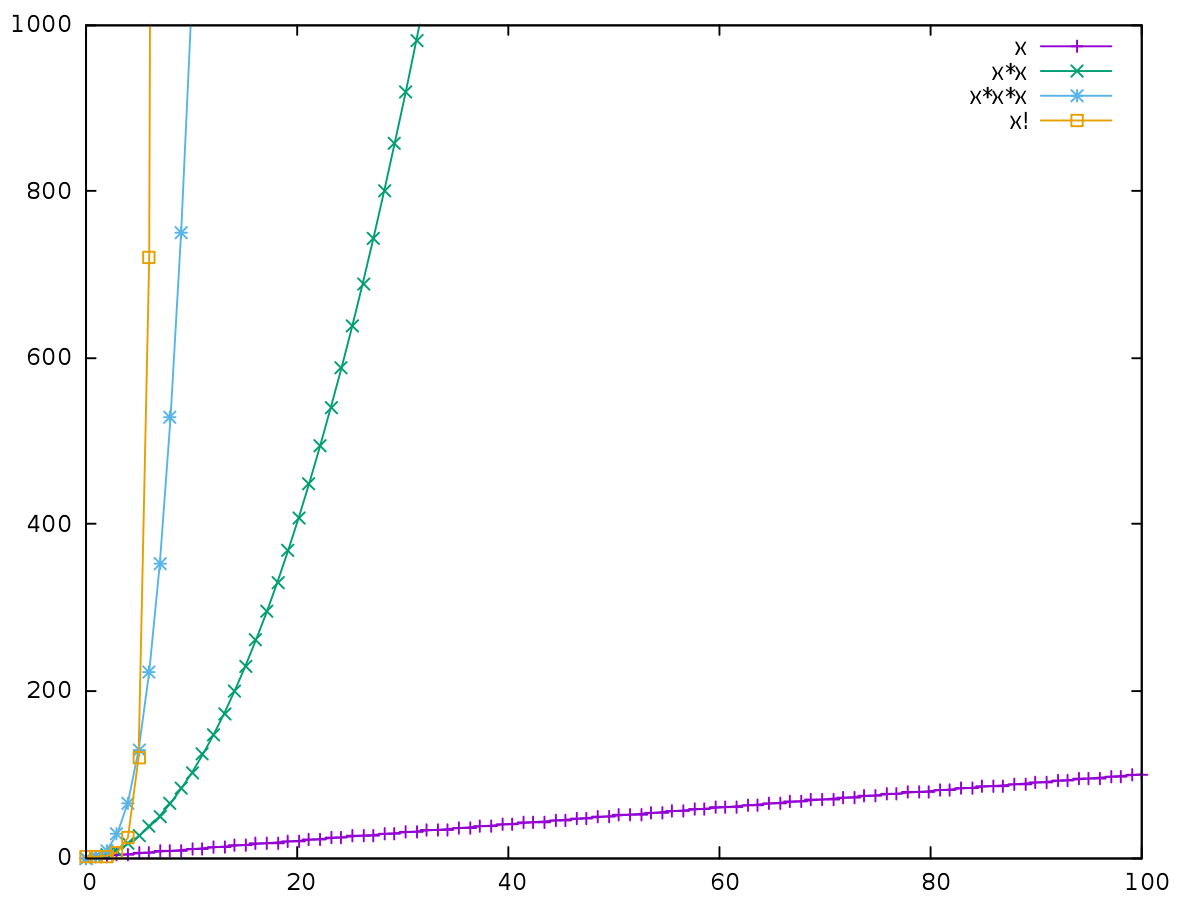
\includegraphics[width=9cm]{fig/graf.png}
			\caption{Crescimento de diferentes funções.}
	  	\label{label}
	  \end{figure}
	\end{frame}
	
	
	\section{Exemplo: Bubble Sort}
	
		
	\begin{frame}[c]{Exemplo: Ordenação}
	
		\begin{block}{Problema da Ordenação}
		Ordenação é o ato de se colocar os elementos de uma sequência de informações, ou dados, em uma ordem predefinida.
		\end{block}

		\begin{enumerate}
			\item Algoritmo Bubble Sort (Bolha)??
			\begin{enumerate}
				\item Fazer trocas sucessivas dois a dois até que o maior elemento esteja na última posição;
				\item Repetir $n-1$ vezes.
			\end{enumerate}

		\end{enumerate}
		
	\end{frame}

	\begin{frame}[fragile]{Bubble Sort - Análise}

		\begin{minted}[
				frame=lines,
				framesep=2mm,
				baselinestretch=1.2,
				%fontsize=\footnotesize,
				linenos
			]{c}
for(i=1; i < n; i++){
	for(j=0; j < n - i; j++){
		if(v[j] > v[j+1])
			// troca v[j] com v[j+1]
			tmp = v[j];
			v[j] = v[j+1];
			v[j+1] = aux;
	}
}
		\end{minted}

			\only<1>{Quantas comparações entre os elementos o algoritmo Bubble Sort realiza?}
			\only<2>{Comparações: $\displaystyle \sum_{i=1}^{n-1}{\sum_{j=0}^{(n-i-1)}{1}}$\\}
	\end{frame}
			
	\begin{frame}[c]{Bubble Sort - Quantidade de Comparações}

		\begin{itemize}[label={}]

			\item[]<1->{$\displaystyle \sum_{i=1}^{n-1}{\sum_{j=0}^{(n-i-1)}{1}}$\\}
			\item[]<2->{$\displaystyle = \sum_{i=1}^{n-1}{(n-i)}$\\}
			\item[]<3->{$\displaystyle = \sum_{i=1}^{n-1}{n} - \sum_{i=1}^{n-1}{i}$\\}
			\item[]<4->{$\displaystyle = (n^2-n) - \frac{(n-1)n}{2}$\\}
			\item[]<5->{$\displaystyle = n^2-n - \frac{n^2-n}{2}$\\}
			\item[]<6->{$\displaystyle = \frac{n^2}{2} - \frac{n}{2} \approx n^2$\\}
		
		\end{itemize}

	\end{frame}
	
	\begin{frame}[c]{Bubble Sort - Quantidade de Comparações}
		Por que $\displaystyle = \frac{n^2}{2} - \frac{n}{2} \approx n^2$?
	\end{frame}
	
	\begin{frame}[c]{Bubble Sort - Quantidade de Comparações}

		\begin{table}
			\centering
			\caption{Crescimento de diferentes funções}
			\begin{tabular}{r|r|r|r}
				\toprule
				\multicolumn{1}{r|}{$n$} & \multicolumn{1}{r|}{$n/2$} & \multicolumn{1}{r|}{$n^{2}/2$} & \multicolumn{1}{r}{$n^{2}$}  \\
				\hline
				64                         & 32                           & 512                               & 1024                            \\
				\hline
				128                        & 64                           & 2048                              & 4096                            \\
				\hline
				512                        & 256                          & 131072                            & 262144                          \\
				\hline
				1024                       & 512                          & 524288                            & 1048576                         \\
				\hline
				2048                       & 1024                         & 2097152                           & 4194304                         \\
				\hline
				4096                       & 2048                         & 8388608                           & 16777216                        \\
				\hline
				8192                       & 4096                         & 33554432                          & 67108864                        \\
				\hline
				16384                      & 8192                         & 134217728                         & 268435456                       \\
				\hline
				32768                      & 16384                        & 536870912                         & 1073741824                      \\
				\bottomrule
			\end{tabular}
		\end{table}
	\end{frame}

	\begin{frame}[c]{Bubble Sort - Quantidade de Comparações}
		\begin{itemize}
			\item $\frac{n^2}{2}$ é o termo dominante quando $n$ é grande;
			\item De um modo geral, podemos nos concentrar nos termos dominantes e esquecer os demais;
			\item Mas sempre devemos pensar quando o valor de $n$ é grande;
		\end{itemize}

		\begin{block}
		``Problema pequeno qualquer algoritmo resolve.'' :)
		\end{block}
	\end{frame}

	\begin{frame}[fragile]{Bubble Sort - Análise Trocas}

		\begin{minted}[
				frame=lines,
				framesep=2mm,
				baselinestretch=1.2,
				fontsize=\footnotesize,
				linenos
			]{c}
for(i=1; i < n; i++){
	for(j=0; j < n - i; j++){
		if(v[j] > v[j+1])
			// troca v[j] com v[j+1]
			tmp = v[j];
			v[j] = v[j+1];
			v[j+1] = aux;
	}
}
		\end{minted}

			Quantas trocas entre os elementos o algoritmo Bubble Sort realiza?
			\pause
			\begin{itemize}
			\item \textbf{Melhor} caso?
			\item \textbf{Pior} caso?
			\end{itemize}
	\end{frame}
			
	\section{Exemplo: Fibonacci}
		
	\begin{frame}[c]{Série de Fibonacci}

		\begin{center}
			\[ fib(n) =
			\left \{
			\begin{array}{rc}
				0,&\mbox{se}\quad n = 0,\\
				1,&\mbox{se}\quad n = 1,\\
				fib(n-1) + fib(n-2),&\mbox{se}\quad n \ge 2.
			\end{array}
			\right .
			\]
		\end{center}
	\end{frame}

	\begin{frame}[fragile,c]{Algoritmo 1}

		\begin{minted}[
				frame=lines,
				framesep=2mm,
				baselinestretch=1.2,
				%fontsize=\footnotesize,
				linenos
			]{c}
long int fib(long int n)
{
  if(n == 0) return(0);
  if(n == 1) return(1);
  return(fib(n-1) + fib(n-2));
}
		\end{minted}
	
	\end{frame}

	\begin{frame}[fragile,c]{Algoritmo 2}

		\begin{minted}[
				frame=lines,
				framesep=2mm,
				baselinestretch=1.2,
				fontsize=\footnotesize,
				linenos
			]{c}
long int fib(long int n)
{
   long int first = 1, second = 1, next, c, sum;
   sum = 0;
   for ( c = 0 ; c < n ; c++ ){
      if ( c <= 1 )
         next = c;
      else{
         next = first + second;
         first = second;
         second = next;
      }
   }
   return(next);
}
		\end{minted}
	
	\end{frame}

	
	\section{Conclusão}

	% ==========================================
	\begin{frame}
		\frametitle{Considerações Finais}

		Por que falar de tudo isso em um curso de análise e desenvolvimento?
		\begin{itemize}
			\item Sistemas resolvem problemas cada vez mais \textbf{complexos};
			\begin{itemize}
				\item Saber identificar se um problema tem solução computacional ou não;
				\item Exemplo: Como o waze calcula o menor caminho?
				\item Exemplo: BigData.
			\end{itemize}
			\item Entender diferentes técnicas de algoritmos;
			\item Comparar e escolher soluções para um problema;
			\item Enfim, se tornar um programador melhor;
			
		\end{itemize}
		\pause
		
		\vspace{1cm}
		
	\end{frame}
	% ==========================================


	% ==========================================
	% \begin{frame}
	% 	\frametitle{Título}
	% 	\begin{itemize}
	% 		\item Item bla bla bla
	% 	\end{itemize}
	%	  \begin{block}{Título de bloco}
	%		 	Conteúdo do bloco
	%   \end{block}
	% \end{frame}
	% ==========================================

	% ==========================================
	% Exemplo de frame com figura
	% \begin{frame}
	% 	\frametitle{Título}
	%	  \begin{figure}[h]
	%	  	\centering
	%	  	\includegraphics[width=10cm]{paht.png}
	%			\caption{Bla bla bla ...}
	%	  	\label{label}
	%	  \end{figure}
	% \end{frame}
	% ==========================================

	% ==========================================
	% Exemplo de frame com algoritmo
	% \begin{frame}[fragile]
	% 	\frametitle{Título}
	% 	\begin{lstlisting}[language=C]
	% 		#include <stdio.h>
	%
	% 		int main()
	% 		{
	% 		  int a[5];
	%
	% 		  a[0] = 30;
	% 		  a[1] = 25;
	% 		  a[2] = 5;
	% 		  a[3] = 100;
	% 		  a[4] = 1;
	%
	% 		  printf("%d\n",a[1]);
	% 		}
	% 	\end{lstlisting}
	% \end{frame}
	% ==========================================

	% ==========================================
	% Frame para referências
	%\begin{frame}[allowframebreaks]
	%	\frametitle{Referências utilizadas na apresentação}
	%	\bibliography{referencias}
	%\end{frame}
  % ==========================================

\end{document}
